\section{Calculation of the local energy}

At the sampling part we skipped over an important line.

\begin{minted}{python}
  E_local = local_energy_func(dist_s)
\end{minted}

Where we have to calculate the local energy of the quantum system in question. We know that the local energy of a particular sample state $\ket{s}$ can be calculated as

\begin{equation}
  E_{loc} = \displaystyle\frac{\bra{s}H\ket{\psi_{rbm}}}{\braket{s}{\psi_{rbm}}} \; ,
  \label{eq:local_imp}
\end{equation}

but here we will explain in more detail how this is done for the each of the different systems we are looking at. First of all it is important to remember the structure of the input to our function calculating the local energy. We want to vectorize the calculations as much as possible so the input will be all $m$ samples, taken with the Gibbs or Metropolis-Hastings algorithm, together in one array:

\begin{equation}
  \mathbf{S} = \left [ s_0, s_1, \dots, s_m \right] \; .
  \label{eq:Samples_set}
\end{equation}

To calculate the local energy for the Lipkin and Pairing model we need to have the wave function $\ket{\psi__{rbm}}$.

\begin{equation}
  \ket{\Psi_{rbm}} = \alpha_0\ket{\psi_0} + \alpha_1\ket{\psi_1} + \dots + \alpha_n\ket{\psi_n}
\end{equation}

The coefficients can be approximated. If we define $N_i$ as the number of state $\ket{\psi_i}$ in our sample set $\boldsymbol{S}$, then we have.

\begin{equation}
  \ket{\Psi_{rbm}} \approx \frac{N_0}{m}\ket{\psi_0} +\frac{N_1}{m}\ket{\psi_1} +\dots + \frac{N_n}{m}\ket{\psi_n}
\end{equation}

as an approximation of the machine state.

Looking at the different parts of $E_{loc}$ we have for a example state $\ket{b} \in \boldsymbol{S}$ that

\begin{equation}
  \braket{b}{\phi_{rbm}} = \alpha_i ,
\end{equation}

where $i$ would correspond to where the condition $\ket{b} = \ket{\phi_i}$ is fulfilled. To calculate the numerator of $E_{loc}$ we start with

\begin{equation}
  H\ket{\Psi_{rbm}} =  \alpha_0H\ket{\psi_0} + \alpha_1H\ket{\psi_1} + \dots + \alpha_nH\ket{\psi_n}
\end{equation}

The hamiltonian transforms the states into a new one

\begin{equation}
  H\ket{\psi_i} = \beta_{i,0}\ket{\psi_0} + \dots + \beta_{i,n}\ket{\psi_n}
\end{equation}

so we get

\begin{align}
  H\ket{\Psi_{rbm}} = \alpha_0  ( \beta_{0,0}\ket{\psi_0} &+ \dots + \beta_{0,n}\ket{\psi_n}  ) \\
 + \alpha_1  ( \beta_{1,0}\ket{\psi_0} &+ \dots + \beta_{1,n}\ket{\psi_n}  ) \\
&\vdots \\
+ \alpha_n  ( \beta_{n,0}\ket{\psi_0} &+ \dots + \beta_{n,n}\ket{\psi_n}  ) 
\end{align}

We then have that for the example state $\ket{b}$

\begin{equation}
  \bra{b}H\ket{\Psi_{rbm}} = \sum_{i=0}^n \alpha_j\beta_{i,j} \; ,
\end{equation}

where $j$ again is the corresponding state $\ket{b} = \ket{\psi_j}$.

In the practical calculations we will use the approximated coefficients. To do so we first we create an array of basis states.

\begin{minted}{python} 
def create_basis(n, dtype, device):
    basis = torch.tensor(
        list(itertools.product([0, 1], repeat=n)),
        dtype = dtype,
        device= device
    )
    return basis
\end{minted}

where the \mintinline{python}{itertools.product(...)} creates all combinations of 0 and 1 into a array, and the rest is to make into a PyTorch tensor. With the basis in place we can check it against our samples.

\begin{minted}{python}
  
def amplitudes(samples, basis):
    weight = torch.sum(
      torch.all(samples[:, None] == basis, dim = -1), 
      dim=0
    )

    non_zero_weight = weight[weight!=0]
    weight[weight==0] = 1

    mask = torch.where(
      torch.all(samples[:, None] == basis, dim = -1)
    )[1]

    diff_basis = torch.sum(
        torch.logical_xor(basis[:, None], basis), dim=-1
    )[weight!=0]

    return weight, non_zero_weight, mask, diff_basis
\end{minted}

The \mintinline{python}{weight} creates an array of where it has counted how many times each of the basis states appear in the sample set. \mintinline{python}{non_zero_weight} is to prevent division by zero when calculating the local energy when a basis state is not a part of the machine state. The \mintinline{python}{mask} is a tool to only needing to calculate the local energy for each basis state instead of each sample. We then use \mintinline{python}{mask} to extract the local energy of a sample from its matching basis state. Finally \mintinline{python}{diff_basis} checks how many particles excite up or de-excite down between each of the basis states. Using the broadcasting functionality.
\vspace{\baselineskip}
\\
\begin{*equation}
  \mintinline{python}{xor} \left (\begin{bmatrix}
      \ket{\psi_0} \\ \vdots \\ \ket{\psi_n}
    \end{bmatrix}, \; \left [\ket{\psi_0}, \dots , \ket{\psi_n}\right ] \right ) \rightarrow \begin{bmatrix}
    \mintinline{python}{xor} \left (\ket{\psi_0}, \ket{\psi_0} \right ) & \dots & \mintinline{python}{xor} \left (\ket{\psi_0}, \ket{\psi_n} \right ) \\
                                                                     \vdots   &  & \vdots \\
    \mintinline{python}{xor} \left (\ket{\psi_n}, \ket{\psi_0} \right ) & \dots & \mintinline{python}{xor} \left (\ket{\psi_n}, \ket{\psi_n} \right )
    \end{bmatrix}
\end{*equation}
\vspace{\baselineskip}
\\
We then have a approximation of our machine state $\ket{\psi}$ and the analysis of it to calculate the hamiltonian's effect on it. The next steps varies with the hamiltonian of the system.

\subsection{The Lipkin model}

The Lipkin model hamiltonian is defined as

\begin{equation} 
    H = \sum_{p\sigma} \left ( \frac{1}{2} \sigma \varepsilon \right ) \hc{a}{p\sigma}\op{a}{p\sigma} + \frac{V}{2}\sum_{pp'\sigma} \hc{a}{p\sigma} \hc{a}{p'\sigma} \op{a}{p'-\sigma}\op{a}{p-\sigma} + \frac{W}{2} \sum_{pp'\sigma} \hc{a}{p\sigma} \hc{a}{p'-\sigma} \op{a}{p'\sigma}\op{a}{p-\sigma} \; , 
\end{equation}

For a more structured explanation we separate the hamiltonian in three parts:

\begin{align}
  H_{\varepsilon} &= \sum_{p\sigma} \left ( \frac{1}{2} \sigma \varepsilon \right ) \hc{a}{p\sigma}\op{a}{p\sigma}\\ 
  H_V &= \frac{V}{2}\sum_{pp'\sigma} \hc{a}{p\sigma} \hc{a}{p'\sigma} \op{a}{p'-\sigma}\op{a}{p-\sigma}\\
  H_W &= \frac{W}{2} \sum_{pp'\sigma} \hc{a}{p\sigma} \hc{a}{p'-\sigma} \op{a}{p'\sigma}\op{a}{p-\sigma}  \; .
  \label{eq:LMG_split_H}
\end{align}

 A state $\ket{b}$ contributes for the different parts as follows:

\begin{itemize}
  \item $H_{\varepsilon}$ - the same state $\ket{b}$.
  \item $H_V$ - states that are a excited or de-excited pair away from the state $\ket{b}$.
  \item $H_W$ - states one excited or de-excited particle away from $\ket{b}$.
\end{itemize}

We separate the different parts then sum them together at the end.

\begin{minted}{python}

def lipkin_local(eps, V, W, samples, basis):
    weight, non_zero_weight, mask = amplitudes(samples, basis)

    N_0 = torch.sum(basis == 0, dim=-1)
    N_1 = torch.sum(basis == 1, dim=-1)

    diff_basis = torch.sum(
        torch.logical_xor(basis[:, None], basis), dim=-1
    )[weight!=0]
    
    H_0 = 0.5*eps*(N_1-N_0)
    H_eps = H_0[mask]

    H_1 = V*torch.sum(non_zero_weight[:, None]*(diff_basis == 2), dim=0)/weight
    H_V = H_1[mask]
    
    H_2 = W*torch.sum(non_zero_weight[:, None]*(diff_basis == 1), dim=0)/weight
    H_W = H_2[mask]
    
    E = (H_eps - H_V - H_W)
    return E

\end{minted}

For the $H_{\varepsilon}$ contribution we start of by calculating the number of particles in the first and second layer.

\begin{minted}{python}
    N_0 = torch.sum(unique == 0, dim=-1)
    N_1 = torch.sum(unique == 1, dim=-1)
\end{minted}

The particles in the first layer contribute with negative spin and the particles in the second layer contribute positively, so we get that.

\begin{minted}{python} 
    H_0 = 0.5*eps*(N_1-N_0)
\end{minted}

We then have an array of the machine states amplitudes multiplied by $\varepsilon$. Applying \mintinline{python}{mask} to this array then selects the correct value for each sample without having to calculate duplicates more than once. We then have the $H_{\varepsilon}$ contribution for each sample directly:

\begin{minted}{python} 
    H_eps = H_0[mask]
\end{minted}

We then calculate the difference between the basis states of the machine state, which is the states in \mintinline{python}{unique}, and the number of particles that change layer.

\begin{minted}{python}
    H_1 = V*torch.sum(
      non_zero_weight[:, None]*(diff_basis == 2), 
      dim=0
    )/weight
\end{minted}

Here it is important to notice that even if we only take the contribution of $H\ket{\psi_i}$ where $\ket{\psi_i} \in \ket{\psi_{rbm}}$ the transformed state can contain a basis state that is not a part of the machine state. Hence the removing of zero-valued amplitudes in the \mintinline{python}{weight} array is necessary. If we assume that the machine state contains every basis state for simplicity we have that:
\vspace{\baselineskip}
\\
\begin{equation*}
  \begin{gathered}
    \mintinline{python}{ non_zero_weight[:, None]*(diff_basis == 2)} \rightarrow \boldsymbol{M}_{diff, 2} \\
    \\
    \boldsymbol{M}_{diff, 2} = \begin{bmatrix}
      N_0 \mintinline{python}{xor} \left (\ket{\psi_0}, \ket{\psi_0} \right ) & \dots & N_0  \mintinline{python}{xor} \left (\ket{\psi_0}, \ket{\psi_n} \right ) \\
      \vdots & & \vdots \\
      N_n  \mintinline{python}{xor} \left (\ket{\psi_n}, \ket{\psi_0} \right ) & \dots & N_n  \mintinline{python}{xor} \left (\ket{\psi_n}, \ket{\psi_n} \right )
    \end{bmatrix}
  \end{gathered}
\end{equation*}
\vspace{\baselineskip}
\\
And we have that $\bra{b}H\ket{\Psi_{rbm}} = \sum_{i=0}^n \alpha_j\beta_{i,j}$, so we add the rows together, which is the first dimension in python. We then divide by each of the basis states amplitude before transformation by the hamiltonian. The \mintinline{python}{mask} is then applied:

\begin{minted}{python}
    H_V = H_1[mask]
\end{minted}

For $H_W$ we have the exact same approach, only changing the condition of number of excited or de-excited particles to $1$:

\begin{minted}{python}
    H_2 = W*torch.sum(
      non_zero_weight[:, None]*(diff_basis == 1),
      dim=0
    )/weight
    H_W = H_2[mask]
\end{minted}

And lastly we subtract all the parts as defined in the full Lipkin hamiltonian:

\begin{minted}{python}
    E = (H_eps - H_V - H_W)
    return E
\end{minted}

which we return as an array of the local energy of each of the input samples.

\subsection{The Ising model}

For the Ising model we can calculate the local energy directly with:

\begin{equation}
  H(\boldsymbol{\sigma}) = J\sum_{<i,j>}\sigma_i\sigma_j + L \sum_i \sigma_i \; ,
  \label{eq:imp_hamil_ising}
\end{equation}

where $J$ is the interaction strength between nearest neighbors, and $L$ is the single particle energy against an external field. To calculate this efficiently we take the whole set and shift it:

\begin{minted}{python}
  def ising_local(samples):
    spin = 2*samples - 1
    shifted = torch.roll(spin, dim=1)
\end{minted}

where we then assume the boundary conditions:

\begin{equation}
  \mathbf{\sigma}_0 = \mathbf{\sigma}_N \; ,
  \label{eq:ising_boundary_imp}
\end{equation}

as explained in \ref{sec:ising_theory}. We can then easily calculate the energy of the configuration with a sum:

\begin{minted}{python}
    H_J = J*torch.sum(shifted*spin, dim=1)
    H_L = L*torch.sum(spin, dim=1)
    return H_J + H_L
\end{minted}

where $H_J$ is the interaction part and $H_L$ is the external field part. The Ising model becomes drastically more interesting in higher dimensions, and we will look at the 2-dimensional Ising as well. We just expand our approach of shifting the input array. Practically the input will be a flattened array of the 2-dimensional grid.

\begin{minted}{python}
def ising_2d(samples, J, L):
    
    pm = 2*samples - 1
    size = int(torch.sqrt(pm.shape)[0])
    pm = torch.reshape(pm, (size, size))

    up = torch.roll(pm, 1, 0)
    right = torch.roll(pm, 1, 1)

    H_J = J*torch.sum(up*pm+right*pm)
    H_L = L*torch.sum(pm)

    return H_L + H_J
\end{minted}

The closest neighbours in a grid is on both sides on the same row, and up and down on the column, but to not count pairs twice we only need to roll once in each direction. Reshaping the input we can use the \mintinline{python}{torch.roll(...)} function to shift the matrix in each of these directions, and then multiply and sum them together.

\subsection{The Heisenberg model}

The Heisenberg model's difference to the Ising model is the input, we go from binary spin to continuous, so we reuse the Ising model hamiltonians for both one and two dimensions. To change to continuous spin we use the \mintinline{python}{given_v} instead of the \mintinline{python}{binary} from the layer sampling functions described in the section about the solver.

\subsection{The Pairing model}

 The Pairing model hamiltonian can be written as

\begin{equation}
  \hat{H} = \epsilon \sum_{p\sigma} \left(p-1\right)\hc{a}{p\sigma}\op{a}{p\sigma} - \frac{1}{2}g\sum_{pq}\hat{P}_p^+\hat{P}_q^-
  \label{eq:Pairing_model_imp}
\end{equation}

Where we have that

\begin{equation*}
  \begin{gathered}
    \hat{P}_p^+ = \hc{a}{p+}\hc{a}{p-}\\
    \hat{P}_p^- = \op{a}{p-}\op{a}{p+}
  \end{gathered}
\end{equation*}

First of we need to define how we will represent the states in the RBM's visual layer. In contrast to the Lipkin model, here we always have pairs moving together, so what we will do is have a $1$ in the visual layer represent one such pair. An example state

$$\ket{b} = \left[\;1, 0, 1, 0 \; \right]^T \; ,$$

would visually look like:

\vspace{\baselineskip}
\\
\begin{figure}[H]
  \begin{center}
    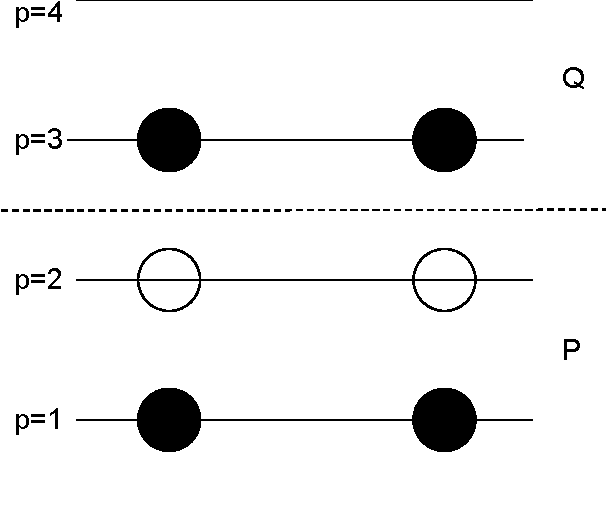
\includegraphics[width=0.5\textwidth]{Figures/Drawn/Pairing/pairing_imp_exp.pdf}
  \end{center}
\end{figure}

We add the size of the model space to a function adjusting a standard basis to accommodate our criteria:

\begin{minted}{python}  
def pairing_cutoff(basis, P):
    mask = torch.sum(basis, dim=-1) == 2*P
    pairing_basis = basis[mask]

    return pairing_basis
\end{minted}

where we only include states where the number of particles is equal to the capacity of the model space. The excluded space is then deduced from the size of the visual layer, though it is not directly used. Further we define our function:

\begin{minted}{python}
def pairing_local_energy(eps, g, samples, basis):    
    weight, non_zero_weight, mask, diff_basis = amplitudes(samples, basis)
\end{minted}

We then find the single particle energy contribution by summing over $(p-1)$ as the spin is already combined. Because of this we need to multiply each contribution by $2$.

\begin{minted}{python} 
    H_0 = 2*eps*torch.sum(torch.where(basis==1), dim=-1) 
    H_eps = H_0[mask]
\end{minted}

In the model description $p$ starts at one, but since array indexing starts at zero we can sum directly without adjustments. Similar to the Lipkin model we can check for changes by using the \minintline{python}{diff_basis} matrix:

\begin{minted}{python}
    H_1 = 0.5*g*torch.sum(
      non_zero_weight[:, None]*(diff_basis==1),
      dim=0
    )/weight
    H_V = H_1[mask]
\end{minted}

where we scale it with the $\frac{1}{2}g$ as defined in the hamiltonian. We then combine them and return the local energies:

\begin{minted}{python}
    E = H_0 - H_V
    return E
\end{minted}


